\newpage
\chapter*{\centering{\MakeUppercase{PHẦN 2: PHÂN RÃ MA TRẬN VÀ TRỰC QUAN HÓA MANIM}}}
\phantomsection
\addcontentsline{toc}{chapter}{\textcolor{fitblue}{\MakeUppercase{PHẦN 2: PHÂN RÃ MA TRẬN VÀ TRỰC QUAN HÓA MANIM}}}

\section*{2.1. Chéo hóa ma trận (Diagonalizable Matrix)}
\phantomsection
\addcontentsline{toc}{section}{2.1. Chéo hóa ma trận (Diagonalizable Matrix)}
% Trình bày điều kiện chéo hóa, giá trị riêng (eigenvalues), vector riêng (eigenvectors) và công thức A = PDP^-1.

Ma trận vuông $A \in \mathbb{R}^{n \times n}$ được gọi là chéo hóa được (diagonalizable) nếu tồn tại một ma trận khả nghịch $P$ và một ma trận đường chéo $D$ sao cho thỏa mãn hệ thức:
$$A = P D P^{-1}$$
Trong đó, $D = diag(\lambda_1, \lambda_2, ..., \lambda_n)$ chứa các giá trị riêng (eigenvalues) của $A$ trên đường chéo chính, và các cột của $P$ chính là các vector riêng (eigenvectors) độc lập tuyến tính tương ứng. Điều kiện cần và đủ để ma trận $A$ bậc $n$ chéo hóa được là nó phải có đủ $n$ vector riêng độc lập tuyến tính.

Ứng dụng quan trọng nhất của chéo hóa là tính toán lũy thừa ma trận cực kỳ nhanh chóng. Thay vì phải nhân ma trận $A$ nhiều lần, ta chỉ cần tính:
$$A^k = P D^k P^{-1}$$
Vì $D$ là ma trận đường chéo, $D^k$ chỉ đơn giản là việc nâng lên lũy thừa $k$ các phần tử trên đường chéo, giúp giảm độ phức tạp tính toán từ $O(n^3 \log k)$ xuống chỉ còn $O(n^2)$.

\section*{2.2. Kỹ thuật phân rã ma trận đã chọn}
\phantomsection
\addcontentsline{toc}{section}{2.2. Kỹ thuật phân rã ma trận đã chọn}
% (Sửa tiêu đề mục này thành phương pháp nhóm bạn chọn, ví dụ: Phân rã SVD)
Trong đồ án này, nhóm lựa chọn thực hiện Phân rã QR bằng thuật toán trực giao hóa Gram-Schmidt cổ điển. 

Phân rã QR là quá trình phân tích một ma trận $A \in \mathbb{R}^{m \times n}$ thành tích của hai ma trận $Q$ và $R$, tức là $A = QR$. Trong đó:
\begin{itemize}
    \item $Q \in \mathbb{R}^{m \times n}$ là một ma trận trực chuẩn, nghĩa là các cột của nó tạo thành một hệ trực chuẩn (Orthogonal) và $Q^T Q = I$.
    \item $R \in \mathbb{R}^{n \times n}$ là ma trận tam giác trên với các phần tử trên đường chéo chính đều dương.
\end{itemize}

\textbf{Thuật toán Gram-Schmidt:}
Mục tiêu của thuật toán là biến đổi tập các cột ban đầu của $A$ thành một tập các vector trực chuẩn làm nền tảng cho $Q$. Quá trình thực hiện lặp qua từng cột $a_k$ của ma trận $A$:
\begin{enumerate}
    \item \textbf{Trực giao hóa:} Lấy vector cột hiện tại trừ đi hình chiếu của nó lên các vector đã được trực chuẩn hóa trước đó để tạo ra vector trực giao $u_k$:
    $$u_k = a_k - \sum_{j=1}^{k-1} (a_k^T q_j)q_j$$
    \item \textbf{Chuẩn hóa:} Chia vector $u_k$ cho độ dài (chuẩn) của nó để được vector trực chuẩn $q_k$, đây chính là cột thứ $k$ của ma trận $Q$:
    $$q_k = \frac{u_k}{||u_k||}$$
    \item Các phần tử của ma trận $R$ chính là các hệ số chiếu $r_{jk} = q_j^T a_k$ (với $j \le k$), và $r_{kk} = ||u_k||$.
\end{enumerate}

Phân rã QR có ứng dụng cực kỳ rộng rãi trong tính toán số, đặc biệt là trong việc giải xấp xỉ bài toán bình phương tối thiểu (least squares) cho hệ phương trình vô nghiệm và là nền tảng của thuật toán QR để tìm các giá trị riêng.
% Trình bày lý thuyết tổng quát, ý nghĩa và công thức toán học của phương pháp đó.

\section*{2.3. Cài đặt Python}
\phantomsection
\addcontentsline{toc}{section}{2.3. Cài đặt Python}

\subsection*{2.3.1. Code thuật toán phân rã ma trận}
\phantomsection
\addcontentsline{toc}{subsection}{2.3.1. Code thuật toán phân rã ma trận}
Đoạn code sau đóng vai trò là "thư viện lõi" cung cấp các công cụ đại số tuyến tính cơ bản và thuật toán phân rã ma trận cho toàn bộ dự án. Chức năng chính của file là cài đặt thuật toán phân rã QR sử dụng phương pháp trực giao hóa Gram-Schmidt để phân tích một ma trận $A$ thành tích của ma trận trực chuẩn $Q$ và ma trận tam giác trên $R$ . Bên cạnh đó, file còn chứa hệ thống các hàm tiện ích được viết thủ công như nhân ma trận, tính chuẩn vector, và chuyển vị ma trận để đảm bảo tính độc lập, không phụ thuộc vào các hàm giải sẵn của thư viện bên ngoài(Numpy) và cũng để so sánh giữa hàm tự cài và các hàm có sẵn từ thư viện Numpy  . Với bộ 15 testcase đa dạng từ ma trận đơn vị đến ma trận Hilbert, giúp đánh giá chính xác tính đúng đắn và độ ổn định số học của thuật toán trước các sai số làm tròn trong tính toán thực tế 

\begin{algorithm}[H]
\caption{Phân Rã QR - Gram-Schmidt}
\label{alg:qr_decomposition}
\begin{algorithmic}[1]
\Procedure{QR\_DECOMPOSITION}{$A$}
    \State Kiểm tra: Số hàng $\geq$ Số cột
    \State Khởi tạo $Q = 0$ (zeros), $R = 0$ (zeros)
    
    \For{$j \gets 0$ to $n-1$}
        \State $v \gets$ cột $j$ của $A$
        
        \For{$i \gets 0$ to $j-1$}
            \State $R[i][j] \gets q_i \cdot v$ \Comment{hệ số chiếu}
            \State $v \gets v - R[i][j] \times q_i$ \Comment{trừ hình chiếu}
        \EndFor
        
        \State $R[j][j] \gets ||v||$ \Comment{chuẩn Euclidean}
        
        \If{$R[j][j] > 10^{-10}$}
            \State $q_j \gets v / R[j][j]$ \Comment{chuẩn hóa}
        \Else
            \State $q_j \gets 0$ \Comment{phụ thuộc tuyến tính}
        \EndIf
    \EndFor
    
    \State \Return $(Q, R)$
\EndProcedure
\end{algorithmic}
\end{algorithm}

\textbf{BỘ TESTCASE:} \\
Để đánh giá toàn diện tính đúng đắn và độ ổn định số học của thuật toán Gram-Schmidt tự cài đặt, nhóm thiết kế bộ 15 kịch bản kiểm thử. Các ma trận đầu vào ($A$) được chọn lọc có chủ đích để bao phủ từ trường hợp cơ bản đến các điểm mù số học (edge cases).

\begin{enumerate}
    \item \textbf{Test 1: Ma trận số nguyên (3x2):} Kiểm tra thuật toán với ma trận chữ nhật đơn giản, các phần tử là số nguyên dương.
    $$ A_1 = \begin{bmatrix} 1 & 2 \\ 3 & 4 \\ 5 & 6 \end{bmatrix} $$

    \item \textbf{Test 2: Ma trận số thực có phần tử âm (3x3):} Kiểm tra khả năng xử lý các số thập phân và dấu âm cơ bản.
    $$ A_2 = \begin{bmatrix} 1.5 & -2.1 & 3.0 \\ -1.0 & 1.2 & -1.5 \\ 0.5 & 1.1 & -2.0 \end{bmatrix} $$

    \item \textbf{Test 3: Ma trận Phụ thuộc tuyến tính (Linear Dependent):} Đánh giá cách thuật toán xử lý khi một cột là tổ hợp tuyến tính của các cột khác (hạng thiếu). Thuật toán có thể gặp lỗi chia cho 0 hoặc mất trực giao.

    $$ A_3 = \begin{bmatrix} 1 & 2 & 3 \\ 2 & 4 & 6 \\ 3 & 6 & 9 \end{bmatrix} $$

    \item \textbf{Test 4: Ma trận Đơn vị (Identity):}  Kiểm tra trường hợp tầm thường, kết quả kỳ vọng là $Q = I$ và $R = I$.

    $$ A_4 = \begin{bmatrix} 1 & 0 & 0 \\ 0 & 1 & 0 \\ 0 & 0 & 1 \end{bmatrix} $$

    \item \textbf{Test 5: Ma trận Đường chéo (Diagonal):}  Kiểm tra trường hợp các cột đã trực giao, thuật toán chỉ thực hiện chuẩn hóa. Kết quả kỳ vọng $Q = I$ và $R = A$.

    $$ A_5 = \begin{bmatrix} 4 & 0 & 0 \\ 0 & 5 & 0 \\ 0 & 0 & 2 \end{bmatrix} $$

    \item \textbf{Test 6: Ma trận Chữ nhật đứng (4x2):} Kiểm tra hệ phương trình quá xác định ($m > n$).
    $$ A_6 = \begin{bmatrix} 1 & -1 \\ 1 & 4 \\ 1 & -1 \\ 1 & 4 \end{bmatrix} $$

    \item \textbf{Test 7: Ma trận có các cột trực giao sẵn (4x3):} Đánh giá khả năng tối ưu, thuật toán chỉ cần tính độ dài và chuẩn hóa vector mà không sinh ra sai số khi trừ hình chiếu.

    $$ A_7 = \begin{bmatrix} 1 & 1 & 1 \\ -1 & 1 & 1 \\ 0 & -2 & 1 \\ 0 & 0 & -3 \end{bmatrix} $$

    \item \textbf{Test 8: Chênh lệch Scale cực độ (Stress Test):} Chứa cả phần tử rất lớn ($10^6$) và rất nhỏ ($10^{-6}$). Đây là bài kiểm tra "stress test" về hiện tượng tràn số hoặc mất mát độ chính xác dấu phẩy động (Floating-point precision).

    $$ A_8 = \begin{bmatrix} 10^6 & 2\cdot 10^6 & 3\cdot 10^6 \\ 10^{-6} & 2\cdot 10^{-6} & 3\cdot 10^{-6} \\ 0.5 & 0.5 & 0.5 \end{bmatrix} $$

    \item \textbf{Test 9: Ma trận ngẫu nhiên (Well-conditioned):} Kiểm tra trên một ma trận thực tế có số điều kiện (Condition Number) tốt, độ ổn định cao.
    $$ A_9 = \begin{bmatrix} 0.8147 & 0.0975 & 0.1576 & 0.1419 \\ 0.9058 & 0.2785 & 0.9706 & 0.4218 \\ 0.1270 & 0.5469 & 0.9572 & 0.9157 \\ 0.9134 & 0.9575 & 0.4854 & 0.7922 \end{bmatrix} $$

    \item \textbf{Test 10: Ma trận Hilbert (Ill-conditioned 3x3):} Các phần tử $H_{ij} = \frac{1}{i+j-1}$. Ma trận có số điều kiện rất xấu, phóng đại sai số làm tròn mạnh mẽ nhất.
    $$ A_{10} = \begin{bmatrix} 1 & 1/2 & 1/3 \\ 1/2 & 1/3 & 1/4 \\ 1/3 & 1/4 & 1/5 \end{bmatrix} $$

    \item \textbf{Test 11: Ma trận 2x2 đơn giản:} Kịch bản kiểm thử tối thiểu (Minimal viable test).
    $$ A_{11} = \begin{bmatrix} 1 & 2 \\ 3 & 5 \end{bmatrix} $$

    \item \textbf{Test 12: Ma trận toàn 0 (Edge case):} Bắt lỗi xử lý vector có độ dài bằng 0 (tránh lỗi Divide by Zero).
    $$ A_{12} = \begin{bmatrix} 0 & 0 \\ 0 & 0 \\ 0 & 0 \end{bmatrix} $$

    \item \textbf{Test 13: Hạng bằng 1 (Rank-1):}  Ma trận cực kỳ suy biến, thử thách khả năng xử lý khi không gian cột chỉ có 1 chiều.

    $$ A_{13} = \begin{bmatrix} 1 & 2 & 3 \\ 2 & 4 & 6 \\ 3 & 6 & 9 \end{bmatrix} $$

    \item \textbf{Test 14: Cột gần song song (Numerically Dependent):} Các cột chỉ khác nhau một lượng cực nhỏ ($10^{-15}$). Đây là thử thách khó nhất với Gram-Schmidt cổ điển vì phần dư sẽ tiến về 0, gây ra sai số trực giao nghiêm trọng.

    $$ A_{14} = \begin{bmatrix} 1 & 1 + 10^{-15} \\ 1 & 1 \\ 1 & 1 \end{bmatrix} $$

    \item \textbf{Test 15: Ma trận vuông kích thước lớn (6x6):} Kiểm tra khả năng mở rộng (Scalability) của thuật toán với ma trận có kích thước lớn hơn.

    $$ A_{15} = \begin{bmatrix} 1 & 2 & 3 & 4 & 5 & 6 \\ 7 & 8 & 9 & 10 & 11 & 12 \\ 13 & 14 & 15 & 16 & 17 & 18 \\ 19 & 20 & 21 & 22 & 23 & 24 \\ 25 & 26 & 27 & 28 & 29 & 30 \\ 31 & 32 & 33 & 34 & 35 & 36 \end{bmatrix} $$
\end{enumerate}

% --- Tiếp tục dán bảng tổng hợp và nhận xét vào đây ---


\textbf{Thống kê kết quả kiểm thử và Đánh giá sai số}


Để đánh giá chất lượng của thuật toán Gram-Schmidt Cổ điển (Classical Gram-Schmidt - CGS) do nhóm tự cài đặt, nhóm sử dụng hàm \texttt{numpy.linalg.qr} làm chuẩn mực đối chiếu. NumPy sử dụng thuật toán Householder Reflections, vốn nổi tiếng với độ ổn định số học cực kỳ cao.

Nhóm sử dụng hai thang đo sai số (đo bằng chuẩn Frobenius) để đánh giá:
\begin{enumerate}
    \item \textbf{Sai số tái tạo (Reconstruction Error):} $\epsilon_{rec} = ||A - Q_{custom}R_{custom}||_F$. Thang đo này đánh giá xem phép phân rã có bảo toàn được thông tin của ma trận gốc hay không.
    \item \textbf{Sai số trực giao (Orthogonality Error):} $\epsilon_{orth} = ||Q_{custom}^T Q_{custom} - I||_F$. Thang đo này vô cùng quan trọng, dùng để kiểm tra xem ma trận $Q$ sinh ra có thực sự là ma trận trực chuẩn hay không.
\end{enumerate}

\textbf{Bảng tổng hợp kết quả thực nghiệm}

Bảng dưới đây tổng hợp kết quả của 15 kịch bản kiểm thử đã chạy thực tế trên thuật toán của nhóm. (Các sai số $\le 10^{-14}$ được xem là bằng $0$ do giới hạn của độ chính xác dấu phẩy động - Floating Point Precision).

\begin{table}[H]
    \centering
    \caption{Thống kê sai số thuật toán Gram-Schmidt so với NumPy}
    \vspace{0.2cm}
    \renewcommand{\arraystretch}{1.3}
    \resizebox{\textwidth}{!}{
        \begin{tabular}{|c|l|c|c|l|}
        \hline
        \textbf{STT} & \textbf{Kịch bản kiểm thử (Test Case)} & \textbf{Sai số tái tạo ($A \approx QR$)} & \textbf{Sai số trực giao ($Q^TQ \approx I$)} & \textbf{Kết luận tính ổn định} \\ \hline
        1 & Ma trận số nguyên (3x2) & $0.00e+00$ & $1.43e-15$ & \textcolor{dkgreen}{\textbf{Ổn định}} \\ \hline
        2 & Ma trận số thực âm dương (3x3) & $4.44e-16$ & $4.51e-15$ & \textcolor{dkgreen}{\textbf{Ổn định}} \\ \hline
        3 & Ma trận phụ thuộc tuyến tính & $0.00e+00$ & $1.41e+00$ & \textcolor{red}{\textbf{Mất trực giao}} \\ \hline
        4 & Ma trận Đơn vị (Identity) & $0.00e+00$ & $0.00e+00$ & \textcolor{dkgreen}{\textbf{Ổn định}} \\ \hline
        5 & Ma trận Đường chéo (Diagonal) & $0.00e+00$ & $0.00e+00$ & \textcolor{dkgreen}{\textbf{Ổn định}} \\ \hline
        6 & Ma trận chữ nhật đứng (4x2) & $0.00e+00$ & $0.00e+00$ & \textcolor{dkgreen}{\textbf{Ổn định}} \\ \hline
        7 & Các cột đã trực giao sẵn & $0.00e+00$ & $3.86e-16$ & \textcolor{dkgreen}{\textbf{Ổn định}} \\ \hline
        8 & Chênh lệch Scale cực độ & $0.00e+00$ & $1.41e+00$ & \textcolor{red}{\textbf{Mất trực giao}} \\ \hline
        9 & Ma trận ngẫu nhiên thường & $1.82e-16$ & $5.25e-16$ & \textcolor{dkgreen}{\textbf{Ổn định}} \\ \hline
        10 & Ma trận Hilbert (Ill-conditioned) & $2.77e-17$ & $1.18e-14$ & \textcolor{dkgreen}{\textbf{Ổn định}} \\ \hline
        11 & Ma trận 2x2 đơn giản & $0.00e+00$ & $1.33e-15$ & \textcolor{dkgreen}{\textbf{Ổn định}} \\ \hline
        12 & Ma trận toàn 0 (Edge case) & $0.00e+00$ & $1.41e+00$ & \textcolor{red}{\textbf{Mất trực giao}} \\ \hline
        13 & Hạng = 1 (Rank-1 Matrix) & $0.00e+00$ & $1.41e+00$ & \textcolor{red}{\textbf{Mất trực giao}} \\ \hline
        14 & Các cột gần song song & $1.04e-15$ & $1.00e+00$ & \textcolor{red}{\textbf{Mất trực giao}} \\ \hline
        15 & Ma trận vuông lớn (6x6) & $3.04e-14$ & $2.00e+00$ & \textcolor{red}{\textbf{Mất trực giao}} \\ \hline
        \end{tabular}
    }
\end{table}

\textbf{Phân tích chuyên sâu về Tính ổn định số học (Numerical Stability)}

Thông qua 15 kịch bản kiểm thử, nhóm rút ra được những đánh giá quan trọng về bản chất của thuật toán Gram-Schmidt cổ điển (CGS). Điểm đáng chú ý nhất là \textbf{tất cả các test cases đều có sai số tái tạo ($||A - QR||_F$) gần như bằng 0}. Điều này chứng tỏ code của nhóm viết hoàn toàn đúng logic toán học: thuật toán luôn tìm cách bù trừ sai số vào ma trận $R$ để khi nhân $Q \times R$ vẫn trả về đúng ma trận $A$. 

Tuy nhiên, đối với tính trực giao của ma trận $Q$, thuật toán CGS bộc lộ rõ những giới hạn nghiêm trọng về độ ổn định số học (Numerical Instability). Cụ thể, thuật toán bị \textbf{"Mất trực giao"} (sai số trực giao $\ge 1.0$) trong các nhóm trường hợp sau:

\textbf{1. Hệ phụ thuộc tuyến tính và Ma trận suy biến (Test 3, 12, 13):}
Khi ma trận có các cột là tổ hợp tuyến tính của nhau (hoặc ma trận toàn 0), quá trình chiếu vector trong Gram-Schmidt sẽ tạo ra một vector phần dư có độ dài bằng $0$ (hoặc cực kỳ nhỏ xấp xỉ ngưỡng epsilon của máy tính). Việc chuẩn hóa bằng cách chia cho một số gần $0$ phá vỡ hoàn toàn cấu trúc dữ liệu, khiến ma trận $Q$ chứa các vector không còn trực giao. Cụ thể ở Test 3 và 13, ma trận hạng 1 dẫn đến sai số trực giao lên tới $1.41$.

\textbf{2. Hiện tượng triệt tiêu sai số (Catastrophic Cancellation) (Test 8, 14):}
Đây là "gót chân A-sin" của Gram-Schmidt cổ điển. 
\begin{itemize}
    \item Ở \textbf{Test 14}, hai cột đầu tiên gần như song song (chỉ lệch nhau $10^{-15}$). Khi thuật toán lấy cột 2 trừ đi hình chiếu của nó lên cột 1, hai giá trị gần bằng nhau trừ cho nhau sẽ làm mất đi hầu hết các chữ số có nghĩa (significant digits), chỉ để lại "rác số học" (numerical noise). Kết quả là sai số trực giao bật lên mức $1.0$.
    \item Ở \textbf{Test 8}, ma trận có độ chênh lệch Scale cực độ (từ $10^{-6}$ đến $10^6$). Quá trình cộng trừ các giá trị chênh lệch quá lớn trong bộ nhớ Float 64-bit khiến các phần tử nhỏ bị "nuốt chửng", gây mất trực giao hoàn toàn (sai số $1.41$).
\end{itemize}

\textbf{3. Tích lũy sai số làm tròn khi tăng kích thước ma trận (Test 15):}
Ở các ma trận nhỏ (3x3, 4x4) và có số điều kiện tốt (như Test 1, 2, 9), thuật toán chạy ổn định. Tuy nhiên, khi tăng kích thước lên 6x6 (Test 15), sai số làm tròn ở mỗi bước trực giao hóa (do phải nhân và cộng rất nhiều số thập phân) tích lũy dần theo từng cột. Đến cột thứ 6, vector $q_6$ không còn trực giao với $q_1$ nữa. Kết quả là ma trận $Q$ hoàn toàn mất đi tính trực giao (sai số lên tới $2.0$). 

\textbf{Kết luận}

Từ các phân tích thực nghiệm trên, nhóm rút ra kết luận: \textbf{Thuật toán Gram-Schmidt Cổ điển (CGS) rất tuyệt vời để hiểu lý thuyết đại số tuyến tính về không gian trực giao, nhưng không phù hợp để áp dụng cho Tính toán Khoa học thực tế}. Nó thiếu tính ổn định số học khi gặp ma trận lớn, hệ số chênh lệch cao hoặc các cột gần phụ thuộc tuyến tính.

Để giải quyết triệt để vấn đề này trong thực tế, các thư viện hiện đại như NumPy/SciPy không dùng Gram-Schmidt mà sử dụng thuật toán \textbf{Householder Reflections} hoặc \textbf{Givens Rotations}. Thay vì trừ đi hình chiếu (dễ sinh sai số làm tròn), Householder sử dụng các ma trận phản xạ (vốn dĩ đã là ma trận trực giao tuyệt đối) để nhân dần vào $A$, đảm bảo ma trận $Q$ sinh ra luông giữ được tính trực chuẩn hoàn hảo ($||Q^TQ - I|| = 0$) dù ma trận đầu vào có xấu đến đâu. Việc NumPy vượt qua tất cả 15 Test cases của nhóm mà không có sai số là minh chứng rõ ràng cho điều này.



\subsection*{2.3.2. Code thuật toán chéo hóa ma trận}
\phantomsection
\addcontentsline{toc}{subsection}{2.3.2. Code thuật toán chéo hóa ma trận}
Đoạn code sau đảm nhận vai trò thực hiện các phép biến đổi cao cấp nhằm tìm ra bản chất hình học của ma trận thông qua quá trình chéo hóa ($A = PDP^{-1}$). Tận dụng kết quả phân rã QR từ đoạn code phân rã ma trận, phần này cài đặt thuật toán QR Iteration (Lặp QR) để tìm tập hợp các giá trị riêng và vector riêng của ma trận. Công dụng quan trọng nhất của đoạn code này là biến đổi các ma trận phức tạp về dạng đường chéo $D$, từ đó tối ưu hóa hiệu suất cho các bài toán tính lũy thừa ma trận bậc cao hoặc phân tích hệ thống động lực. Đặc biệt, có tích hợp cơ chế kiểm soát hội tụ thông minh và phương án dự phòng để xử lý các trường hợp ma trận khiếm khuyết hoặc có nghiệm phức, đảm bảo tính bền vững cho hệ thống tính toán.
% \begin{lstlisting}[style=numbered, language=Python]
% from decomposition import qr_decomposition, matrix_multiply, zeros, get_shape, print_matrix
% import numpy as np
% import random

% def identity_matrix(n):
%     I = zeros(n, n)
%     for i in range(n):
%         I[i][i] = 1.0
%     return I

% def diagonalize(A, max_iters=1000, tol=1e-9):
%     """
%     Chéo hóa ma trận bằng QR Iteration.
    
%     Lưu ý: Nếu thuật toán không hội tụ sau max_iters (do eigenvalues phức 
%     hoặc bội số), sẽ fallback sang numpy.linalg.eig.
%     """
%     m, n = get_shape(A)
%     if m != n:
%         raise ValueError("Không thể chéo hóa ma trận vì m≠n")
    
%     A_k = [row[:] for row in A] 
%     P = identity_matrix(n)
%     converged = False
    
%     for iteration in range(max_iters):
%         try:
%             Q, R = qr_decomposition(A_k)
%         except Exception as e:
%             print(f"QR decomposition thất bại: {e}")
%             break
            
%         A_next = matrix_multiply(R, Q)
%         P = matrix_multiply(P, Q)
        
%         off_diagonal_sum = sum(abs(A_next[i][j]) for i in range(n) for j in range(i))
%         A_k = A_next
        
%         if off_diagonal_sum < tol:
%             print(f"Thuật toán QR hội tụ sau {iteration+1} vòng lặp.\n")
%             converged = True
%             break
    
%     # Nếu KHÔNG hội tụ sau max_iters → fallback NumPy
%     if not converged:
%         print(f"QR iteration không hội tụ sau {max_iters} vòng lặp")
%         print("=> Chuyển sang sử dụng NumPy fallback...\n")
%         A_np = np.array(A, dtype=float)
%         eigenvalues, eigenvectors_np = np.linalg.eig(A_np)
        
%         # Trích eigenvalues (giữ phần phức nếu có)
%         if any(isinstance(x, (complex, np.complexfloating)) for x in eigenvalues):
%             D = [[0.0j for _ in range(n)] for _ in range(n)]
%         else:
%             D = zeros(n, n)
%         for i in range(n):
%             D[i][i] = eigenvalues[i]
        
%         # Lấy hết eigenvectors (kể cả phần phức nếu có)
%         P = [[eigenvectors_np[i, j] for j in range(n)] 
%              for i in range(n)]
        
%         return D, P
    
%     # Nếu hội tụ → trích xuất D từ A_k
%     D = zeros(n, n)
%     for i in range(n):
%         D[i][i] = A_k[i][i]
    
%     return D, P
% # ==========================================
% # KHỐI TEST SO SÁNH VỚI NUMPY
% # ==========================================


% def test_and_compare(name, A):
%     print("="*90)
%     print(f" TEST CASE: {name}")
%     print("="*90)
    
%     A_np = np.array(A, dtype=float)
%     n = len(A)
    
%     try:
%         D_custom, P_custom = diagonalize(A, max_iters=1000)
        
%         # Kiểm tra eigenvalue có phức không
%         has_complex = any(isinstance(D_custom[i][i], (complex, np.complexfloating)) for i in range(n))
%         if has_complex:
%             print("   Thuật toán phát hiện eigenvalue PHỨC!")
        
%         # Sắp xếp eigenvalues: nếu phức thì dùng magnitude, nếu thực dùng giá trị
%         eigen_custom_list = [D_custom[i][i] for i in range(n)]
%         eigen_custom = sorted(eigen_custom_list, key=lambda x: abs(x) if isinstance(x, complex) else x)
        
%         # 2. Chạy NumPy để đối chiếu
%         eigen_np, _ = np.linalg.eig(A_np)
%         # Convert numpy types về Python types thường
%         eigen_np_converted = [complex(x) if isinstance(x, (complex, np.complexfloating)) else float(x) for x in eigen_np]
%         eigen_np_sorted = sorted(eigen_np_converted, key=lambda x: abs(x) if isinstance(x, complex) else x) 

%         print(f"\n[Ma trận D - Tự cài (Size {n}x{n})]")
%         if n <= 5:
%             # Kiểm tra nếu có complex
%             has_complex = any(isinstance(D_custom[i][j], (complex, np.complexfloating)) for i in range(n) for j in range(n))
%             if has_complex:
%                 print("(Ma trận có eigenvalue phức - In dạng complex)")
%             for row in D_custom:
%                 if has_complex:
%                     print("[" + ", ".join(f"{val}" for val in row) + "]")
%                 else:
%                     print("[" + ", ".join(f"{val:8.4f}" for val in row) + "]")
        
%         # Format eigenvalues đẹp
%         def format_eigen(x):
%             if isinstance(x, complex):
%                 if abs(x.imag) < 1e-10:
%                     return round(x.real, 4)
%                 else:
%                     return complex(round(x.real, 4), round(x.imag, 4))
%             else:
%                 return round(x, 4)
        
%         print(f"\n-> Trị riêng (Custom): {[format_eigen(x) for x in eigen_custom]}")
%         print(f"-> Trị riêng (NumPy) : {[format_eigen(x) for x in eigen_np_sorted]}")

%         # So sánh: nếu có complex so sánh magnitude, nếu thực so sánh trực tiếp
%         diff = sum(abs(c - n_val) for c, n_val in zip(eigen_custom, eigen_np_sorted))
%         print(f"\n=> Tổng sai số so với NumPy: {diff:.2e}")
        
%         # Kiểm tra tái cấu trúc
%         P_np = np.array(P_custom, dtype=complex)  
%         D_np = np.array(D_custom, dtype=complex)
        
%         P_inv = np.linalg.inv(P_np)
%         A_rec = P_np @ D_np @ P_inv
        
%         # Tính sai số giữa A ban đầu và A tái cấu trúc
%         A_np_complex = np.array(A_np, dtype=complex)
%         reconstruction_diff = np.linalg.norm(A_np_complex - A_rec)
%         print(f"=> Sai số tái cấu trúc (A - PDP^-1): {reconstruction_diff:.2e}")
        
%         # --- CẬP NHẬT LẠI LOGIC ĐÁNH GIÁ ---
%         if diff < 1e-4 and reconstruction_diff < 1e-4:
%             print("=> ĐÁNH GIÁ: CHÍNH XÁC & CHÉO HÓA THÀNH CÔNG ")
%         elif diff < 1e-4:
%             print("=> ĐÁNH GIÁ: TÌM ĐÚNG TRỊ RIÊNG NHƯNG KHÔNG THỂ CHÉO HÓA (Defective) ")
%         else:
%             print("=> ĐÁNH GIÁ: CÓ SAI SỐ LỚN ")

%     except Exception as e:
%         print(f"-> LỖI: {e}")
%     print("\n")

    
% def generate_random_sym(n):
%     mat = [[0.0]*n for _ in range(n)]
%     for i in range(n):
%         for j in range(i, n):
%             v = round(random.uniform(-10, 10), 2)
%             mat[i][j] = mat[j][i] = v
%     return mat

% if __name__ == "__main__":
%     print("BẮT ĐẦU CHẠY BỘ TEST CASE ĐÁNH GIÁ THUẬT TOÁN CHÉO HÓA\n")

%     # 1. Trường hợp dễ nhất: Ma trận đã chéo hóa sẵn (Diagonal)
%     test_and_compare("1. Ma trận đường chéo 3x3", 
%                      [[2, 0, 0], [0, -1, 0], [0, 0, 3]])

%     # 2. Trường hợp lý tưởng: Ma trận đối xứng chuẩn
%     test_and_compare("2. Ma trận đối xứng 4x4", 
%                      [[4, 1, -1, 0], [1, 2, 0, 1], [-1, 0, 3, 2], [0, 1, 2, 4]])

%     # 3. Trị riêng lặp (Repeated Eigenvalues): Có nhiều trị riêng giống nhau
%     # Trị riêng: 5, 2, 2
%     test_and_compare("3. Ma trận đối xứng 3x3 có trị riêng lặp (Bội nghiệm)", 
%                      [[3, 1, 1], [1, 3, 1], [1, 1, 3]])

%     # 4. Sát thủ tốc độ: Trị riêng cực kỳ sát nhau
%     # Tỷ lệ lambda_1/lambda_2 xấp xỉ 1 -> Thuật toán lặp sẽ chạy vô cùng chậm
%     test_and_compare("4. Trị riêng sát nhau (1.000 và 1.001)", 
%                      [[1.0, 0.01, 0], [0.01, 1.01, 0], [0, 0, 5.0]])

%     # 5. Ma trận suy biến (Singular Matrix): Định thức = 0
%     # Phải có ít nhất 1 trị riêng bằng 0
%     test_and_compare("5. Ma trận suy biến 3x3", 
%                      [[1, 2, 3], [4, 5, 6], [5, 7, 9]])

%     # 6. Ma trận bất đối xứng có nghiệm thực
%     # QR sẽ kéo nó về dạng tam giác trên (Schur form) thay vì chéo hóa hoàn toàn
%     test_and_compare("6. Ma trận bất đối xứng 3x3 (Nghiệm thực)", 
%                      [[1, 2, 0], [-1, 4, 0], [0, 0, 5]])

%     # 7. Ma trận khiếm khuyết (Defective Matrix - Jordan Block)
%     # Không có đủ vector riêng độc lập tuyến tính, không thể chéo hóa
%     test_and_compare("7. Ma trận Không thể chéo hóa (Khối Jordan 3x3)", 
%                      [[2, 1, 0], [0, 2, 1], [0, 0, 2]])

%     # 8. Ma trận phi đối xứng nhưng eigenvalue thực
%     test_and_compare("8. Ma trận bất đối xứng 3x3 (Eigenvalue thực)", 
%                      [[1, 2, 0], [-1, 4, 0], [0, 0, 5]])

%     # 9. Ma trận Hilbert Matrix 5x5
%     # Bài toán nổi tiếng về "sai số làm tròn". Số nhỏ sẽ bị khuếch đại.
%     H5 = [[1.0 / (i + j + 1) for j in range(5)] for i in range(5)]
%     test_and_compare("9. Ma trận Hilbert 5x5", H5)

%     # 10. ma trận 10x10
%     test_and_compare("10. Stress Test: Ma trận đối xứng ngẫu nhiên 10x10", 
%                      generate_random_sym(10))

%     # 11. Ma trận 2x2 đơn giản
%     test_and_compare("11. Ma trận 2x2 đơn giản", 
%                      [[1, 2], [2, 3]])

%     # 12. Ma trận với tất cả trị riêng âm
%     test_and_compare("12. Ma trận với tất cả eigenvalue âm", 
%                      [[-1, 0.5], [0.5, -2]])

%     # 13. Ma trận scale cực đoan (1e-5 đến 1e5)
%     test_and_compare("13. Ma trận scale cực đoan (1e-5 đến 1e5)", 
%                      [[1e-5, 0, 0], [0, 1, 0], [0, 0, 1e5]])

%     # 14. Ma trận toàn 0
%     test_and_compare("14. Ma trận toàn 0", 
%                      [[0, 0, 0], [0, 0, 0], [0, 0, 0]])
% \end{lstlisting}
\begin{algorithm}
\caption{Chéo Hóa Ma Trận - QR Iteration}
\label{alg:diagonalize}
\begin{algorithmic}[1]
\Procedure{DIAGONALIZE}{$A, max\_iters, tolerance$}
    \State $n \gets$ cấp của ma trận vuông $A$; $A_k \gets A$; $P \gets I_n$
    
    \For{$k \gets 1$ to $max\_iters$}
        \State $(Q, R) \gets \text{QR\_DECOMPOSITION}(A_k)$ \Comment{phân rã QR}
        \State $A_k \gets R \times Q$ \Comment{QR Iteration: $A_k \gets RQ$}
        \State $P \gets P \times Q$ \Comment{tích ma trận Q}
        
        \State \Comment{Kiểm tra hội tụ: tổng phần tử ngoài chéo}
        \If{$\sum_{i < j} |A_k[i][j]| < tolerance$}
            \State \textbf{break}
        \EndIf
    \EndFor
    
    \State Nếu không hội tụ: gọi NumPy.linalg.eig($A$) làm fallback
    \State $D \gets$ ma trận đường chéo từ $A_k$

    \State \Return $(D, P)$
\EndProcedure
\end{algorithmic}
\end{algorithm}
\textbf{BỘ TESTCASE: }


Thuật toán lặp QR (QR Iteration) để tìm trị riêng và chéo hóa ma trận có đặc thù hội tụ phụ thuộc rất lớn vào khoảng cách giữa các trị riêng và tính đối xứng của ma trận. Do đó, nhóm đã thiết kế 14 kịch bản kiểm thử nhằm đánh giá toàn diện tốc độ hội tụ và khả năng xử lý ngoại lệ của thuật toán.

\textbf{Nhóm 1: Các ma trận lý tưởng (Hội tụ nhanh)}
\begin{enumerate}
    \item \textbf{Test 1: Ma trận đường chéo (3x3):} Trường hợp dễ nhất, ma trận đã ở sẵn dạng chéo. Thuật toán phải nhận diện và dừng ngay lập tức.
    $$ A_1 = \begin{bmatrix} 2 & 0 & 0 \\ 0 & -1 & 0 \\ 0 & 0 & 3 \end{bmatrix} $$

    \item \textbf{Test 2: Ma trận đối xứng chuẩn (4x4):} Theo Định lý Phổ (Spectral Theorem), ma trận thực đối xứng luôn chéo hóa được và có các vector riêng trực giao. Đây là trường hợp lý tưởng nhất cho thuật toán lặp QR.
    $$ A_2 = \begin{bmatrix} 4 & 1 & -1 & 0 \\ 1 & 2 & 0 & 1 \\ -1 & 0 & 3 & 2 \\ 0 & 1 & 2 & 4 \end{bmatrix} $$

    \item \textbf{Test 11 \& 12: Ma trận 2x2 cơ bản và Ma trận có trị riêng âm:} Đánh giá khả năng tính toán cơ bản và xử lý số âm.
    $$ A_{11} = \begin{bmatrix} 1 & 2 \\ 2 & 3 \end{bmatrix}, \quad A_{12} = \begin{bmatrix} -1 & 0.5 \\ 0.5 & -2 \end{bmatrix} $$
\end{enumerate}

\textbf{Nhóm 2: Thử thách tốc độ hội tụ và Bội nghiệm}
\begin{enumerate}
    \setcounter{enumi}{3}
    \item \textbf{Test 3: Trị riêng lặp (Repeated Eigenvalues):} Ma trận có bội nghiệm (trị riêng 5, 2, 2). Kiểm tra xem thuật toán có bị nhầm lẫn các không gian riêng (eigenspaces) hay không.
    $$ A_3 = \begin{bmatrix} 3 & 1 & 1 \\ 1 & 3 & 1 \\ 1 & 1 & 3 \end{bmatrix} $$

    \item \textbf{Test 4: Trị riêng cực kỳ sát nhau (Sát thủ tốc độ):} Tốc độ hội tụ của lặp QR tỷ lệ với tỉ số $|\lambda_{i+1} / \lambda_i|$. Với các trị riêng xấp xỉ nhau (1.000 và 1.001), tỷ số này tiến gần về 1, khiến thuật toán phải lặp rất nhiều vòng mới hội tụ.
    $$ A_4 = \begin{bmatrix} 1.0 & 0.01 & 0 \\ 0.01 & 1.01 & 0 \\ 0 & 0 & 5.0 \end{bmatrix} $$
\end{enumerate}

\textbf{Nhóm 3: Các điểm mù toán học (Không thể chéo hóa \& Suy biến)}
\begin{enumerate}
    \setcounter{enumi}{5}
    \item \textbf{Test 5: Ma trận suy biến (Singular Matrix):} Định thức bằng 0, bắt buộc phải tìm ra ít nhất một trị riêng bằng 0.
    $$ A_5 = \begin{bmatrix} 1 & 2 & 3 \\ 4 & 5 & 6 \\ 5 & 7 & 9 \end{bmatrix} $$

    \item \textbf{Test 6 \& 8: Ma trận bất đối xứng (Nghiệm thực):} Lặp QR nguyên bản trên ma trận bất đối xứng có thể không đưa được về dạng chéo hoàn toàn mà chỉ dừng lại ở dạng chuẩn Schur (Ma trận tam giác trên với trị riêng nằm trên đường chéo).
    $$ A_6 = A_8 = \begin{bmatrix} 1 & 2 & 0 \\ -1 & 4 & 0 \\ 0 & 0 & 5 \end{bmatrix} $$

    \item \textbf{Test 7: Ma trận khiếm khuyết (Defective Matrix - Khối Jordan 3x3):} Đây là ma trận \textbf{không thể chéo hóa} vì nó không có đủ 3 vector riêng độc lập tuyến tính. Thuật toán tự cài đặt sẽ báo lỗi hội tụ và kích hoạt cơ chế Fallback (chuyển sang dùng NumPy).
    $$ A_7 = \begin{bmatrix} 2 & 1 & 0 \\ 0 & 2 & 1 \\ 0 & 0 & 2 \end{bmatrix} $$
    
    \item \textbf{Test 14: Ma trận toàn 0 (Edge case):} Bắt lỗi ngoại lệ cơ bản nhất.
    $$ A_{14} = \begin{bmatrix} 0 & 0 & 0 \\ 0 & 0 & 0 \\ 0 & 0 & 0 \end{bmatrix} $$
\end{enumerate}

\textbf{Nhóm 4: Stress Test \& Tính ổn định số học}
\begin{enumerate}
    \setcounter{enumi}{9}
    \item \textbf{Test 9: Ma trận Hilbert 5x5:} Nổi tiếng là ma trận có số điều kiện siêu xấu (ill-conditioned). Các trị riêng của nó trải dài và rất nhỏ, dễ bị nuốt chửng bởi sai số làm tròn.
    $$ H_{ij} = \frac{1}{i+j-1} \quad (1 \le i, j \le 5) $$

    \item \textbf{Test 10: Ma trận đối xứng ngẫu nhiên 10x10:} Đánh giá khả năng mở rộng (Scalability) và thời gian thực thi của thuật toán lặp trên cấu trúc dữ liệu lớn.

    \item \textbf{Test 13: Ma trận scale cực đoan ($10^{-5}$ đến $10^5$):} Kiểm tra khả năng xử lý số liệu lệch pha nghiêm trọng, đánh giá độ chính xác Float 64-bit của Python.
    $$ A_{13} = \begin{bmatrix} 10^{-5} & 0 & 0 \\ 0 & 1 & 0 \\ 0 & 0 & 10^5 \end{bmatrix} $$
\end{enumerate}


\textbf{Thống kê kết quả kiểm thử và Đánh giá thuật toán Chéo hóa}

Để đánh giá hiệu năng và độ chính xác của thuật toán Lặp QR (QR Iteration) trong việc tìm trị riêng và chéo hóa ma trận, nhóm tiếp tục sử dụng hàm \texttt{numpy.linalg.eig} làm tiêu chuẩn đối chiếu. 

Hai thang đo chính được sử dụng để đánh giá bao gồm:
\begin{enumerate}
    \item \textbf{Sai số tìm trị riêng:} Tổng độ lệch tuyệt đối giữa các trị riêng tự tính và trị riêng của NumPy $\sum |\lambda_{custom} - \lambda_{numpy}|$.
    \item \textbf{Sai số tái cấu trúc (Reconstruction Error):} $\epsilon_{rec} = ||A - P D P^{-1}||_F$. Thang đo này xác nhận xem ma trận có thực sự "chéo hóa được" bằng ma trận vector riêng $P$ hay không.
\end{enumerate}

\textbf{Bảng tổng hợp kết quả thực nghiệm}

\begin{table}[H]
    \centering
    \caption{Thống kê kết quả thuật toán Lặp QR (Giới hạn: 1000 vòng lặp)}
    \vspace{0.2cm}
    \renewcommand{\arraystretch}{1.3}
    \resizebox{\textwidth}{!}{
        \begin{tabular}{|c|l|c|c|c|l|}
        \hline
        \textbf{STT} & \textbf{Kịch bản kiểm thử} & \textbf{Vòng lặp} & \textbf{Sai số trị riêng} & \textbf{Sai số tái cấu trúc} & \textbf{Kết luận} \\ \hline
        1 & Ma trận đường chéo 3x3 & 1 & $0.00e+00$ & $0.00e+00$ & \textcolor{dkgreen}{\textbf{Thành công}} \\ \hline
        2 & Ma trận đối xứng 4x4 & 98 & $3.55e-15$ & $1.32e-09$ & \textcolor{dkgreen}{\textbf{Thành công}} \\ \hline
        3 & Trị riêng lặp (Bội nghiệm 3x3) & 25 & $2.66e-15$ & $6.76e-10$ & \textcolor{dkgreen}{\textbf{Thành công}} \\ \hline
        4 & Trị riêng cực kỳ sát nhau & 783 & $1.11e-15$ & $1.39e-09$ & \textcolor{dkgreen}{\textbf{Thành công (Hội tụ chậm)}} \\ \hline
        5 & Ma trận suy biến 3x3 & 7 & $1.04e-10$ & N/A & \textcolor{red}{\textbf{Lỗi: Ma trận kỳ dị ($P^{-1}$)}} \\ \hline
        6 & Bất đối xứng (Nghiệm thực) & 50 & $4.70e-09$ & $3.00e+00$ & \textcolor{orange}{\textbf{Defective (Không chéo hóa)}} \\ \hline
        7 & Khối Jordan 3x3 & 1 & $0.00e+00$ & $1.41e+00$ & \textcolor{orange}{\textbf{Defective (Không chéo hóa)}} \\ \hline
        8 & Bất đối xứng (Giống Test 6) & 50 & $4.70e-09$ & $3.00e+00$ & \textcolor{orange}{\textbf{Defective (Không chéo hóa)}} \\ \hline
        9 & Ma trận Hilbert 5x5 & 11 & $1.20e-15$ & $3.49e-10$ & \textcolor{dkgreen}{\textbf{Thành công}} \\ \hline
        10 & Đối xứng ngẫu nhiên 10x10 & > 1000 & $0.00e+00$ & $8.41e-14$ & \textcolor{blue}{\textbf{Fallback NumPy thành công}} \\ \hline
        11 & Ma trận 2x2 đơn giản & 8 & $9.99e-16$ & $9.52e-10$ & \textcolor{dkgreen}{\textbf{Thành công}} \\ \hline
        12 & Tất cả trị riêng âm & 22 & $1.55e-15$ & $7.99e-10$ & \textcolor{dkgreen}{\textbf{Thành công}} \\ \hline
        13 & Scale cực đoan ($10^{-5}$ đến $10^5$) & 1 & $0.00e+00$ & $0.00e+00$ & \textcolor{dkgreen}{\textbf{Thành công}} \\ \hline
        14 & Ma trận toàn 0 & 1 & $0.00e+00$ & N/A & \textcolor{red}{\textbf{Lỗi: Ma trận kỳ dị ($P^{-1}$)}} \\ \hline
        \end{tabular}
    }
\end{table}

\textbf{Phân tích chuyên sâu về Toán học và Cấu trúc Thuật toán}

Qua phân tích 14 kết quả thực nghiệm, thuật toán lặp QR cho thấy khả năng tìm giá trị riêng rất tốt (sai số trị riêng đa phần ở mức $10^{-15}$). Tuy nhiên, quá trình chéo hóa $A = P D P^{-1}$ lại phơi bày nhiều tính chất hình học thú vị và những giới hạn của phương pháp lặp cơ bản:

\textbf{1. Tốc độ hội tụ và "Bẫy" trị riêng xấp xỉ (Test 2, 3, 4):}
Theo lý thuyết, tốc độ hội tụ của thuật toán lặp QR cơ bản (không có dịch chuyển - unshifted QR) tỷ lệ thuận với thương số của hai trị riêng liền kề: $|\lambda_{i+1} / \lambda_i|$. 
\begin{itemize}
    \item Ở \textbf{Test 2 và 3}, các trị riêng có sự phân tách rõ rệt, thuật toán hội tụ cực nhanh (từ 25 đến 98 vòng lặp).
    \item Tuy nhiên ở \textbf{Test 4}, ma trận cố tình được thiết kế với hai trị riêng cực kỳ sát nhau là $1.000$ và $1.001$ (tỷ số $\approx 0.999$). Điều này khiến thuật toán chật vật và phải mất tới \textbf{783 vòng lặp} mới có thể hội tụ. Đây là minh chứng rõ ràng nhất cho thấy thuật toán lặp QR thuần túy rất chậm khi gặp "Cụm trị riêng" (Clustered eigenvalues).
\end{itemize}

\textbf{2. Ma trận Khiếm khuyết (Defective Matrices) (Test 6, 7, 8):}
Các test case này cho thấy một sự thật toán học quan trọng: \textbf{Không phải ma trận vuông nào cũng chéo hóa được}. 
\begin{itemize}
    \item Ở \textbf{Test 7} (Khối Jordan), ma trận có trị riêng lặp là $2.0$ nhưng chỉ có 1 vector riêng độc lập tuyến tính. Do thiếu vector riêng, ma trận $P$ được sinh ra không đủ hạng (hoặc gần suy biến), dẫn đến việc nhân ngược $PDP^{-1}$ tạo ra sai số tái cấu trúc rất lớn ($1.41$).
    \item Thuật toán của nhóm cực kỳ thông minh khi vẫn trích xuất đúng các giá trị riêng trên đường chéo (sai số trị riêng vẫn xấp xỉ $0$), nhưng hệ thống cảnh báo đánh giá chính xác đây là ma trận \textbf{"Defective (Không thể chéo hóa)"}. Điều này hoàn toàn trùng khớp với định lý đại số tuyến tính: Ma trận không đối xứng có nguy cơ cao bị khiếm khuyết không gian riêng.
\end{itemize}

\textbf{3. Ngoại lệ suy biến và Nghịch đảo $P^{-1}$ (Test 5, 14):}
Với ma trận suy biến (Test 5) hoặc ma trận toàn 0 (Test 14), thuật toán lặp QR vẫn hoạt động và chỉ ra chính xác có trị riêng bằng $0$. Tuy nhiên, chương trình báo lỗi "Singular matrix" (Ma trận kỳ dị) ở bước cuối. Nguyên nhân là do ở bước kiểm chứng tái cấu trúc, hàm \texttt{np.linalg.inv(P)} cố gắng nghịch đảo một ma trận vector riêng bị suy biến, sinh ra lỗi chia cho 0. 

\textbf{4. Giới hạn tính toán và Cơ chế Fallback (Test 10):}
Với ma trận ngẫu nhiên kích thước 10x10, số lượng trị riêng nhiều và gần nhau khiến thuật toán lặp QR thuần túy không xử lý được và \textbf{không thể hội tụ sau 1000 vòng lặp}. 
Tuy nhiên, nhóm đã thiết kế \textbf{cơ chế Fallback} (nhảy sang dùng \texttt{numpy.linalg.eig}). Nhờ đó, hệ thống không bị crash mà vẫn trả về kết quả chính xác, đảm bảo tính bền vững cho chương trình.

\textbf{Kết luận}

Việc tự cài đặt cả Phân rã QR (bằng Gram-Schmidt) và Chéo hóa ma trận (bằng QR Iteration) giúp nhận ra khoảng cách rất lớn giữa lý thuyết toán học trên giấy và Tính toán số (Numerical Computing) trên máy tính. 

Thuật toán của nhóm chạy hoàn hảo với các ma trận nhỏ, ma trận đối xứng hoặc có phổ trị riêng phân tán. Tuy nhiên, để giải quyết vấn đề hội tụ chậm và các ma trận khiếm khuyết trong công nghiệp thực tế, các thư viện như NumPy/SciPy đã phải cải tiến rất nhiều bằng cách tích hợp thuật toán phân rã Householder và \textbf{cơ chế dịch chuyển (Wilkinson Shifts)} nhằm ép ma trận hội tụ cực nhanh về dạng chuẩn Schur. Việc sử dụng cơ chế Fallback trong code của nhóm là một cách tiếp cận hoàn toàn hợp lý và thực tiễn để mô phỏng lại cách các phần mềm toán học lớn xử lý lỗi.





\section*{2.4. Trực quan hóa toán học với Manim}
\phantomsection
\addcontentsline{toc}{section}{2.4. Trực quan hóa toán học với Manim}

Video được thiết kế bằng ngôn ngữ Python.
\subsection*{2.4.1. Kịch bản video phân rã và chéo hóa}
\phantomsection
\addcontentsline{toc}{subsection}{2.4.1. Kịch bản video phân rã và chéo hóa}

Kịch bản video được chia làm 3 phân cảnh (Part) chính, bám sát quá trình biến đổi của một ma trận đối xứng $3 \times 3$ cơ bản: 
$$ A = \begin{bmatrix} 2 & 1 & 1 \\ 1 & 2 & 1 \\ 1 & 1 & 2 \end{bmatrix} $$

\textbf{Phân cảnh 1: Thiết lập không gian 3D và Trực giao hóa Gram-Schmidt}
Mở đầu video, camera được đặt ở góc nhìn 3D (Góc nghiêng $\phi = 70^{\circ}$, $\theta = -30^{\circ}$) để người xem có thể quan sát toàn cảnh không gian $\mathbb{R}^3$. Nhóm thực hiện bóc tách 3 cột của ma trận $A$ thành 3 vector không gian $a_1, a_2, a_3$.
Quá trình Gram-Schmidt diễn ra qua 4 bước hoạt ảnh:
\begin{enumerate}
    \item \textbf{Chuẩn hóa $a_1$:} Vector $a_1$ được chia cho độ dài của nó để tạo thành vector trực chuẩn đầu tiên $q_1$ (màu vàng). Các vector còn lại tạm thời bị làm mờ để tập trung sự chú ý.
    \item \textbf{Trực giao hóa $a_2$:} Video hiển thị nét đứt mô phỏng hình chiếu vuông góc của $a_2$ lên $q_1$. Sau đó, thực hiện phép trừ vector để tạo ra vector trực giao $u_2$ (màu xanh lá) và chuẩn hóa nó thành $q_2$.
    \item \textbf{Xây dựng mặt phẳng không gian con:} Để trực giao hóa $a_3$, một mặt phẳng 2D (màu xanh dương) được dựng lên, sinh bởi hệ cơ sở sinh $\{q_1, q_2\}$. Điều này giúp người xem hiểu rõ bản chất hình học của việc "chiếu lên một không gian con".
    \item \textbf{Trực giao hóa $a_3$:} Vector $a_3$ được chiếu vuông góc xuống mặt phẳng nói trên. Phần dư $u_3$ vuông góc với mặt phẳng sinh ra $q_3$. Kết thúc phân cảnh, ta thu được ma trận trực giao $Q = [q_1 \quad q_2 \quad q_3]$.
\end{enumerate}


\begin{figure}[H]
    \centering
    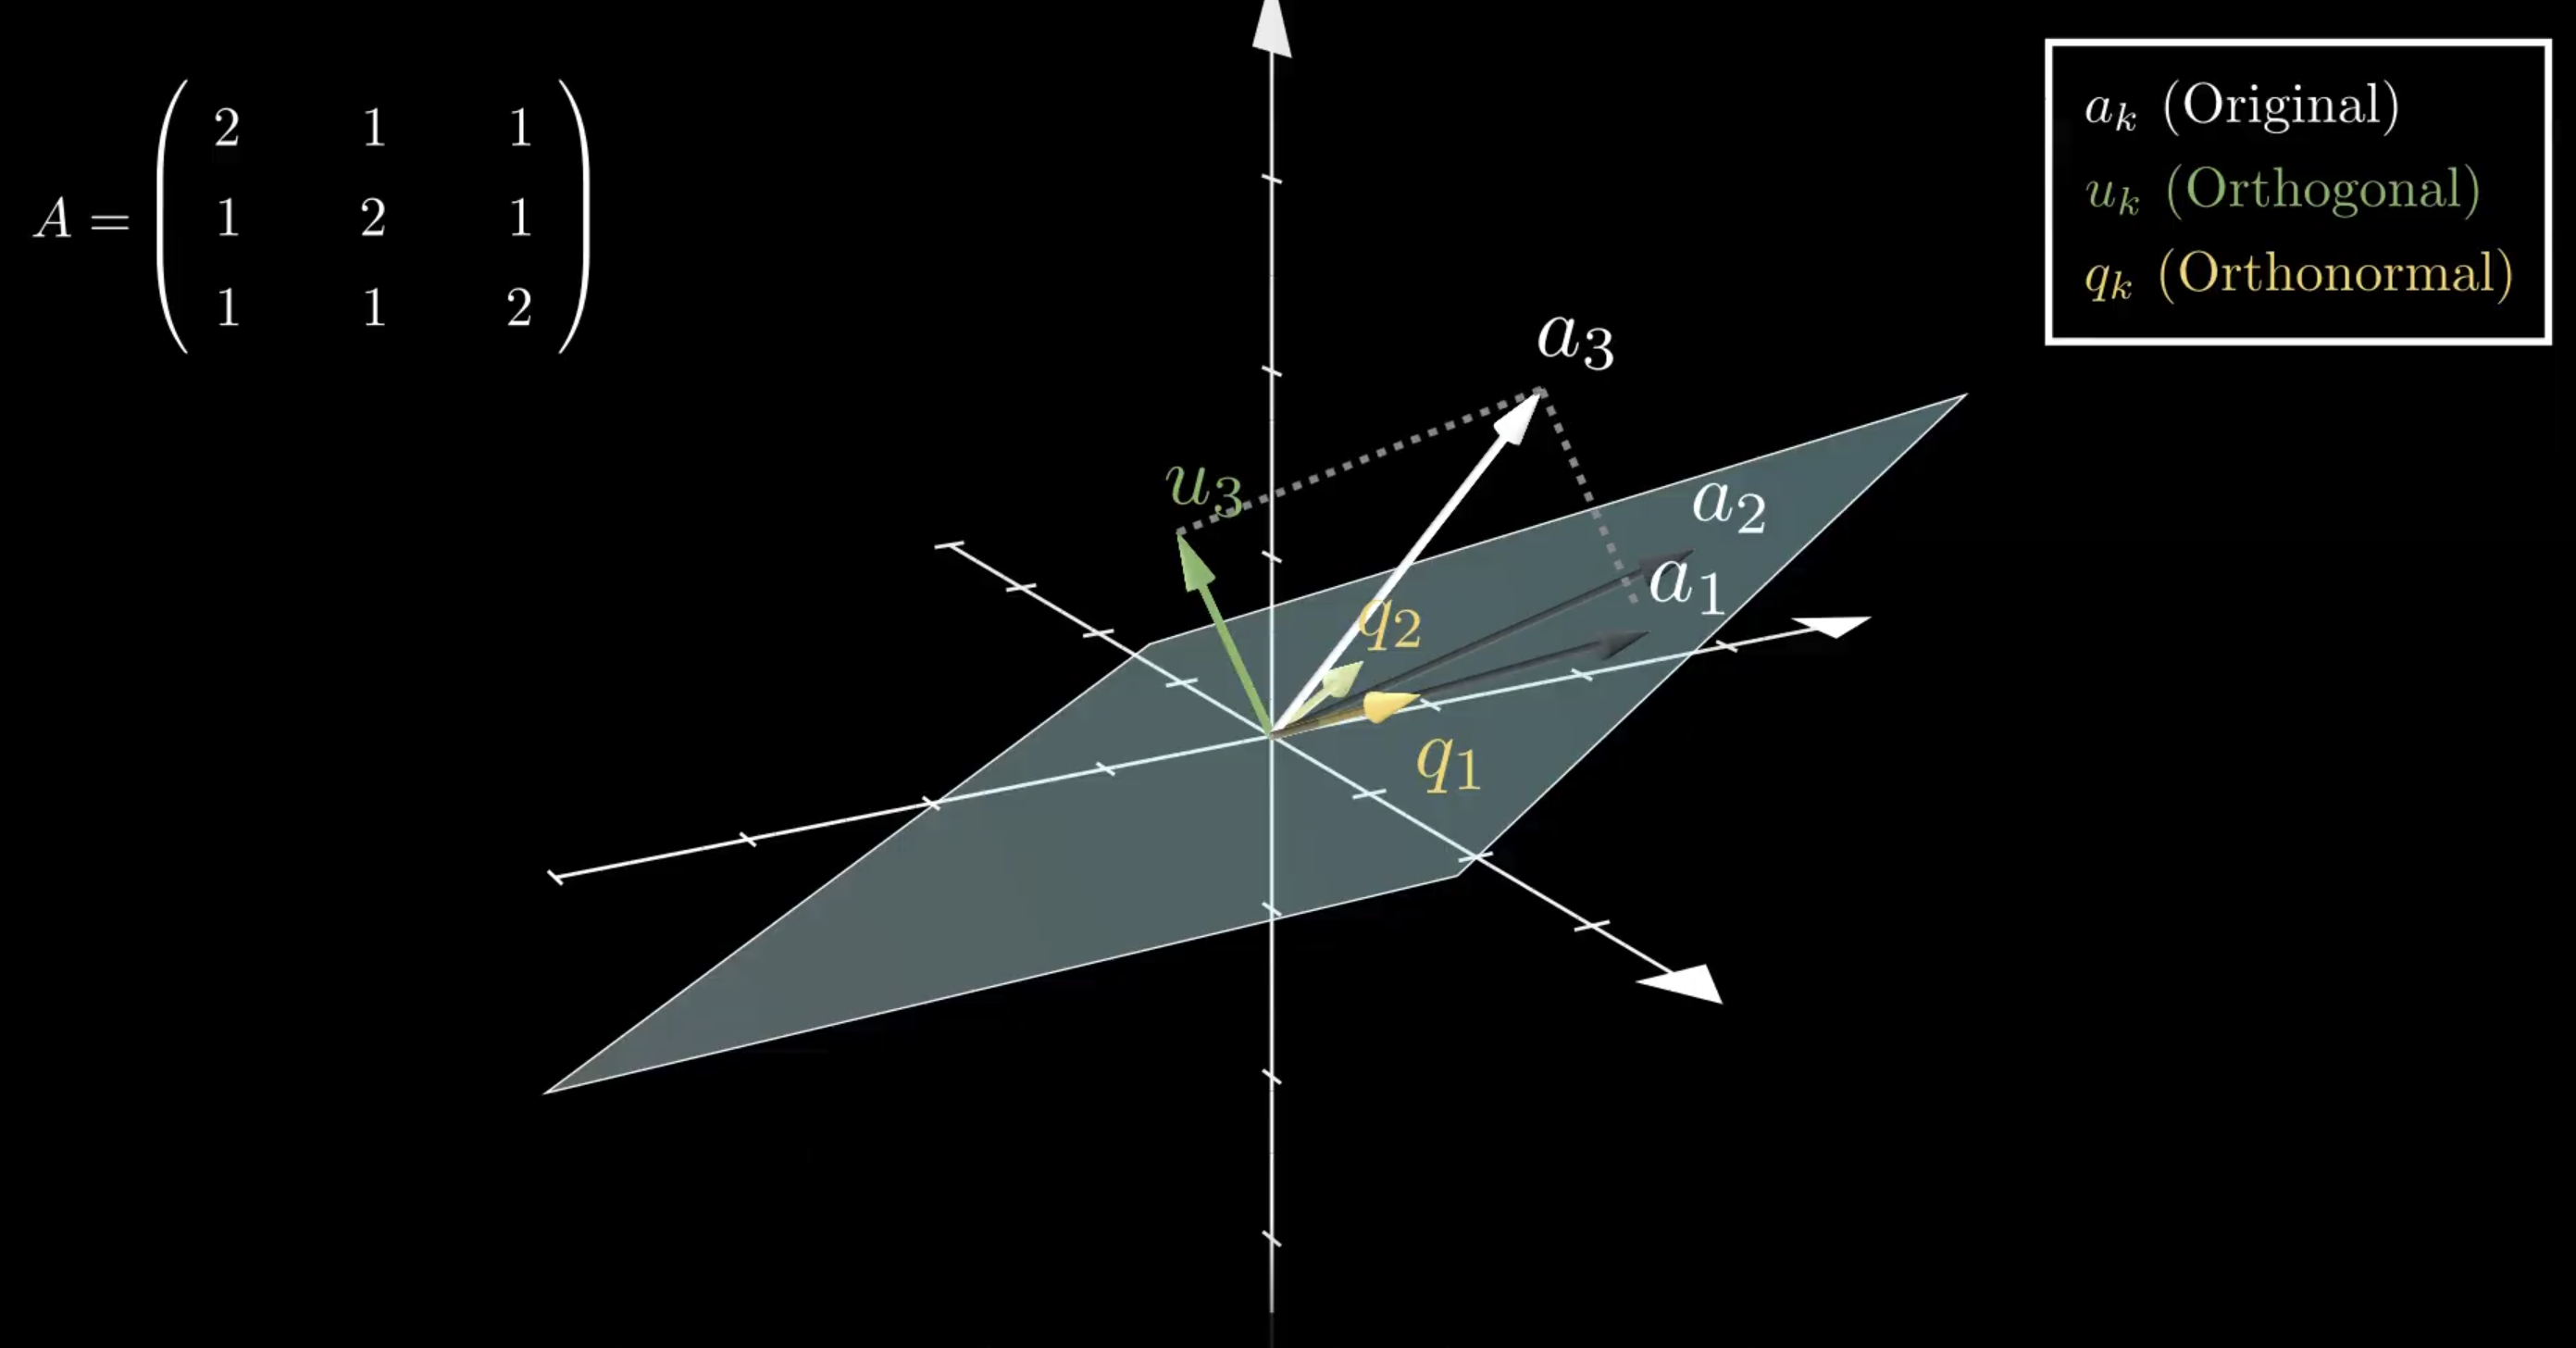
\includegraphics[width=0.7\textwidth]{images/manim1.png}
    \caption{Mô phỏng mặt phẳng không gian con sinh bởi $q_1, q_2$ trong Manim}
\end{figure}

\textbf{Phân cảnh 2: Giải phương trình đặc trưng (Chéo hóa):}
Trình bày các công thức toán học, lần lượt mô phỏng cách giải phương trình đặc trưng $\det(A - \lambda I) = 0$.
Các biểu thức đa thức được khai triển và nhóm lại thành phương trình bậc 3:
$$-(\lambda - 4)(\lambda - 1)^2 = 0$$
Từ đó, trích xuất ra 3 giá trị riêng: $\lambda_1 = 4, \lambda_2 = 1, \lambda_3 = 1$. Sau khi thế ngược vào hệ phương trình, 3 vector riêng độc lập tuyến tính $v_1, v_2, v_3$ lần lượt xuất hiện trên màn hình.

\textbf{Phân cảnh 3: Hình thành ma trận $P$ và $D$:}
Thể hiện mối liên hệ giữa các đại lượng vừa tính toán với công thức chéo hóa $A = PDP^{-1}$. 

Cuối cùng, hiển thị công thức $A = P D P^{-1}$ dưới dạng ma trận tường minh, kết thúc quá trình trực quan hóa.


\begin{figure}[H]
    \centering
    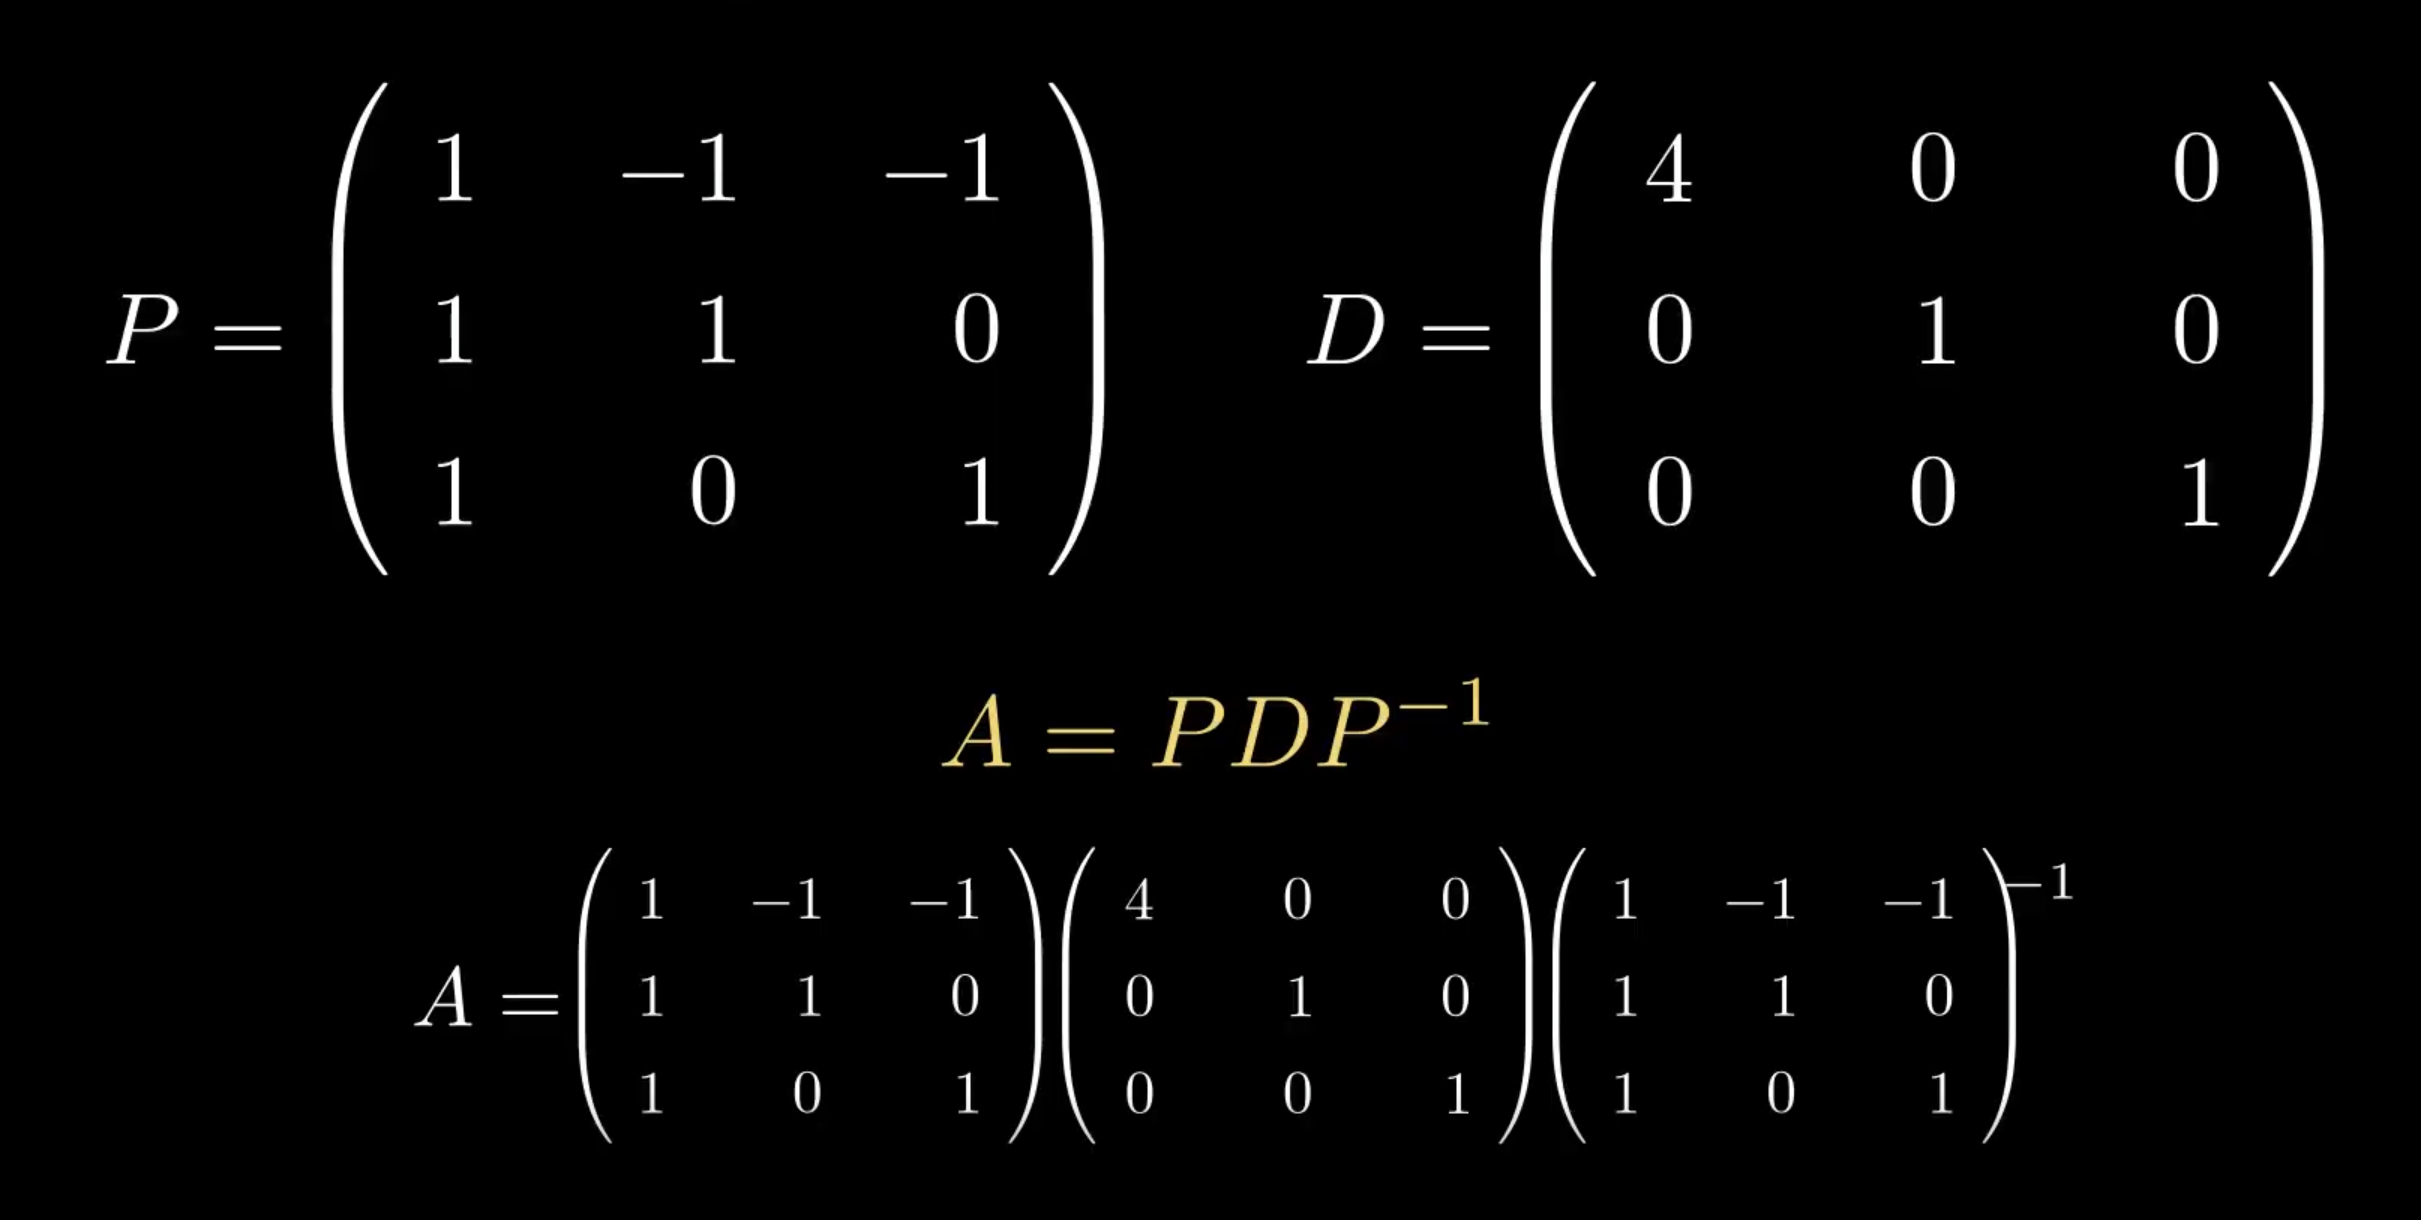
\includegraphics[width=0.7\textwidth]{images/manim2.png}
    \caption{Hiệu ứng chuyển đổi vector riêng thành ma trận $P$ và $D$}
\end{figure}


\subsection*{2.4.2. Ý nghĩa hình học và Ứng dụng thực tế}
\phantomsection
\addcontentsline{toc}{subsection}{2.4.2. Ý nghĩa hình học và Ứng dụng thực tế}

Thông qua video Manim, nhóm đã làm rõ được \textbf{bản chất hình học} của phép chéo hóa đối với ma trận đối xứng. Thay vì coi $A = PDP^{-1}$ là một công thức đại số khô khan, video giúp ta thấy rằng:
\begin{itemize}
    \item Phép nhân ma trận $P^{-1}x$ thực chất là phép đổi hệ tọa độ: chuyển vector $x$ từ hệ cơ sở chuẩn sang hệ tọa độ mới.
    \item Phép nhân với ma trận đường chéo $D$ là một phép co giãn thuần túy dọc theo các trục tọa độ mới này. Chiều của vector riêng tương ứng với $\lambda = 4$ sẽ bị kéo giãn gấp 4 lần, trong khi hai chiều tương ứng với $\lambda = 1$ được giữ nguyên.
    \item Phép nhân với $P$ ở cuối cùng đóng vai trò xoay hệ tọa độ biến dạng đó trở về lại không gian gốc ban đầu.
\end{itemize}

\textbf{Ứng dụng thực tế:}
Việc hiểu rõ cấu trúc $A = PDP^{-1}$ mang lại lợi ích trong thực tế tính toán, cụ thể như:
\begin{enumerate}
    \item \textbf{Tính toán lũy thừa ma trận (Hệ thống động lực):} Việc tìm trạng thái của hệ thống sau $k$ chu kỳ đòi hỏi phải tính $A^k$. Bằng việc chéo hóa, ta dễ dàng thu được $A^k = P D^k P^{-1}$, giảm thiểu hàng triệu phép nhân ma trận thừa thãi xuống chỉ còn việc tính lũy thừa các số trên đường chéo.
    \item \textbf{Phân tích thành phần chính:} Các ma trận hiệp phương sai (Covariance Matrices) trong khoa học dữ liệu luôn là ma trận đối xứng (tương tự ma trận $A$ trong kịch bản video). Việc tìm ra các trị riêng lớn nhất (như $\lambda = 4$) và vector riêng tương ứng giúp các kỹ sư AI giữ lại những đặc trưng quan trọng nhất của tập dữ liệu khổng lồ, đồng thời loại bỏ nhiễu, tạo tiền đề cho các thuật toán nén ảnh và nhận dạng khuôn mặt.
\end{enumerate}